\documentclass[11pt]{article}
\usepackage{fullpage}
\usepackage{enumitem}
\usepackage{pdfpages}
\usepackage{graphicx}
\begin{document}
\author{Benjamin Sorenson} \title{Assignment 3}
\maketitle
\begin{enumerate}[label=\bfseries Question \arabic*:]
\item %question 1
  The last page of this document contains the game tree with
  evaluations.  The starting move is highlighted in green and the
  nodes pruned assuming optimal ordering are highlighted in red.
  \begin{enumerate}
  \item There are \(9!\)
    possible ways to fill-in a tic-tac-toe board---this is an
    overestimate, but a good-enough approximation of the size of the
    search space.
  \end{enumerate}
\item %question 2
  \begin{enumerate}
  \item This will happen when \(e1\)
    is \(b\) times faster than \(e2\).
  \item With \(\alpha\)-\(\beta\)
    pruning, assuming optimal ordering, this will happen when \(e1\)
    is \(\sqrt{b}\)
    times faster than \(e2\),
    and with random ordering, when \(e1\)
    is \(d^{\frac{3}{4}}\) times faster than \(e2\).
  \item With \(\alpha\)-\(\beta\)
    pruning, less dramatic increases in speed get the same or better
    performance increases than you would get in mini-max, but ordering
    is more important than raw speed.  With mini-max, you have to
    visit and evaluate each node so raw speed is more important than
    it is with \(\alpha\)-\(\beta\) pruning.
  \end{enumerate}
\item %question 3
  Constraints:
  \[I \ne D \ne O \ne T\]
  \[I + D = O + C_{10} \cdot 10\]
  \[I + C_{10} = O + C_{100} \cdot 10\]
  \[D + C_{100} = T\]
  \[\forall v \in \{I, D, O, T\}; 0 \le v \le 9\]
  Using the MRC heuristic, we are always assigning values to variables
  with the fewest available legal assignments.
  \begin{enumerate}[label=\bfseries Depth \arabic*:]
  \item assign \(C_{100} = 1\)
    as this is the only legal assignment for \(C_{100}\)
    (assigning \(C_{100}=0\) violates the constraint that \(D \ne T\)
  \item assign \(C_{10} = 1\)
    as this is the only legal assignment (\(C_{10} = 0\)
    violates the constraint that \(I \le 9 \))
  \item assign \(I = 9\)
    as this is the only legal assignment for \(I\)
    since \(I + 1 \ge 10\)
  \item assign \(O = 0\)
    as this is the only legal assignment for \(O\)
    since \(I + 1 = O + 10\)
  \item assign \(D = 1\)
    as this is the only legal assignment for \(D\)
    since \(9 + D = 0 + 10 \)
  \item assign \(T = 2\)
    as this is the only legal assignment for \(T\) since \(1 + 1 = T\)
  \end{enumerate}
\item %question 4
  To answer each part of this question, I will use the fact that the
  size of the search space \(s\)
  in \(n\)
  variables with a set of domains \(D = \{D_1, D_2, \dots D_n\}\)
  is equal to \( \prod_{i=1}^{n}{|D_i|} \).
  From this it follows that the size of \(s\)
  is \(\Omega (d_{\min} ^ n)\)
  and \( O (d_{\max}^n ) \)
  where \(d_{\min} = \min\{|D_i|; D_i \in D\}\)
  and \(d_{\max} = \max\{|D_i|; D_i \in D\}\).
  From this if follows that:
  \begin{enumerate}
  \item The size of \(s\) is exponential in the number of variables
  \item The size of \(s\) is polynomial in the size of the domains.
  \end{enumerate}
\item %question 5
  It is often a good idea to choose the most constrained variable and
  the least constraining value when we are only interested in finding
  the first solution rather than all solutions to a CSP. This is
  because by choosing the most constrained variable, we eliminate all
  the nodes in the search tree where we would run out of possible
  values for the most constrained variable, and by choosing the least
  constraining value for that variable, we eliminate fewer
  possibilities for the remaining variables making it more likely we
  will find a solution.
\item %question 6
  There are 18 possible solutions to the map-coloring problem for the
  Australia map with three colors. Tazmania can take any of the three
  colors regardless of the colors chosen for any of the 6 other
  states. The colors of the rest of the states are driven by the color
  choice of Southern Australia which can take any of the three colors.
  After we have made a choice for Southern Australia, there are really
  only 2 possible remaining solutions---one where Western Australia is
  one of the remaining 2 colors or the other since the only
  restricition is that it can't be the color chosen for Southern
  Australia.  After that choice has been made there is only one
  possible color for each of the remaining states since every state
  other than Tazmania borders Western Australia and one other state.
  This comes out to \(3 \cdot 3 \cdot 2 = 18 \) possible solutions.
 

\end{enumerate}
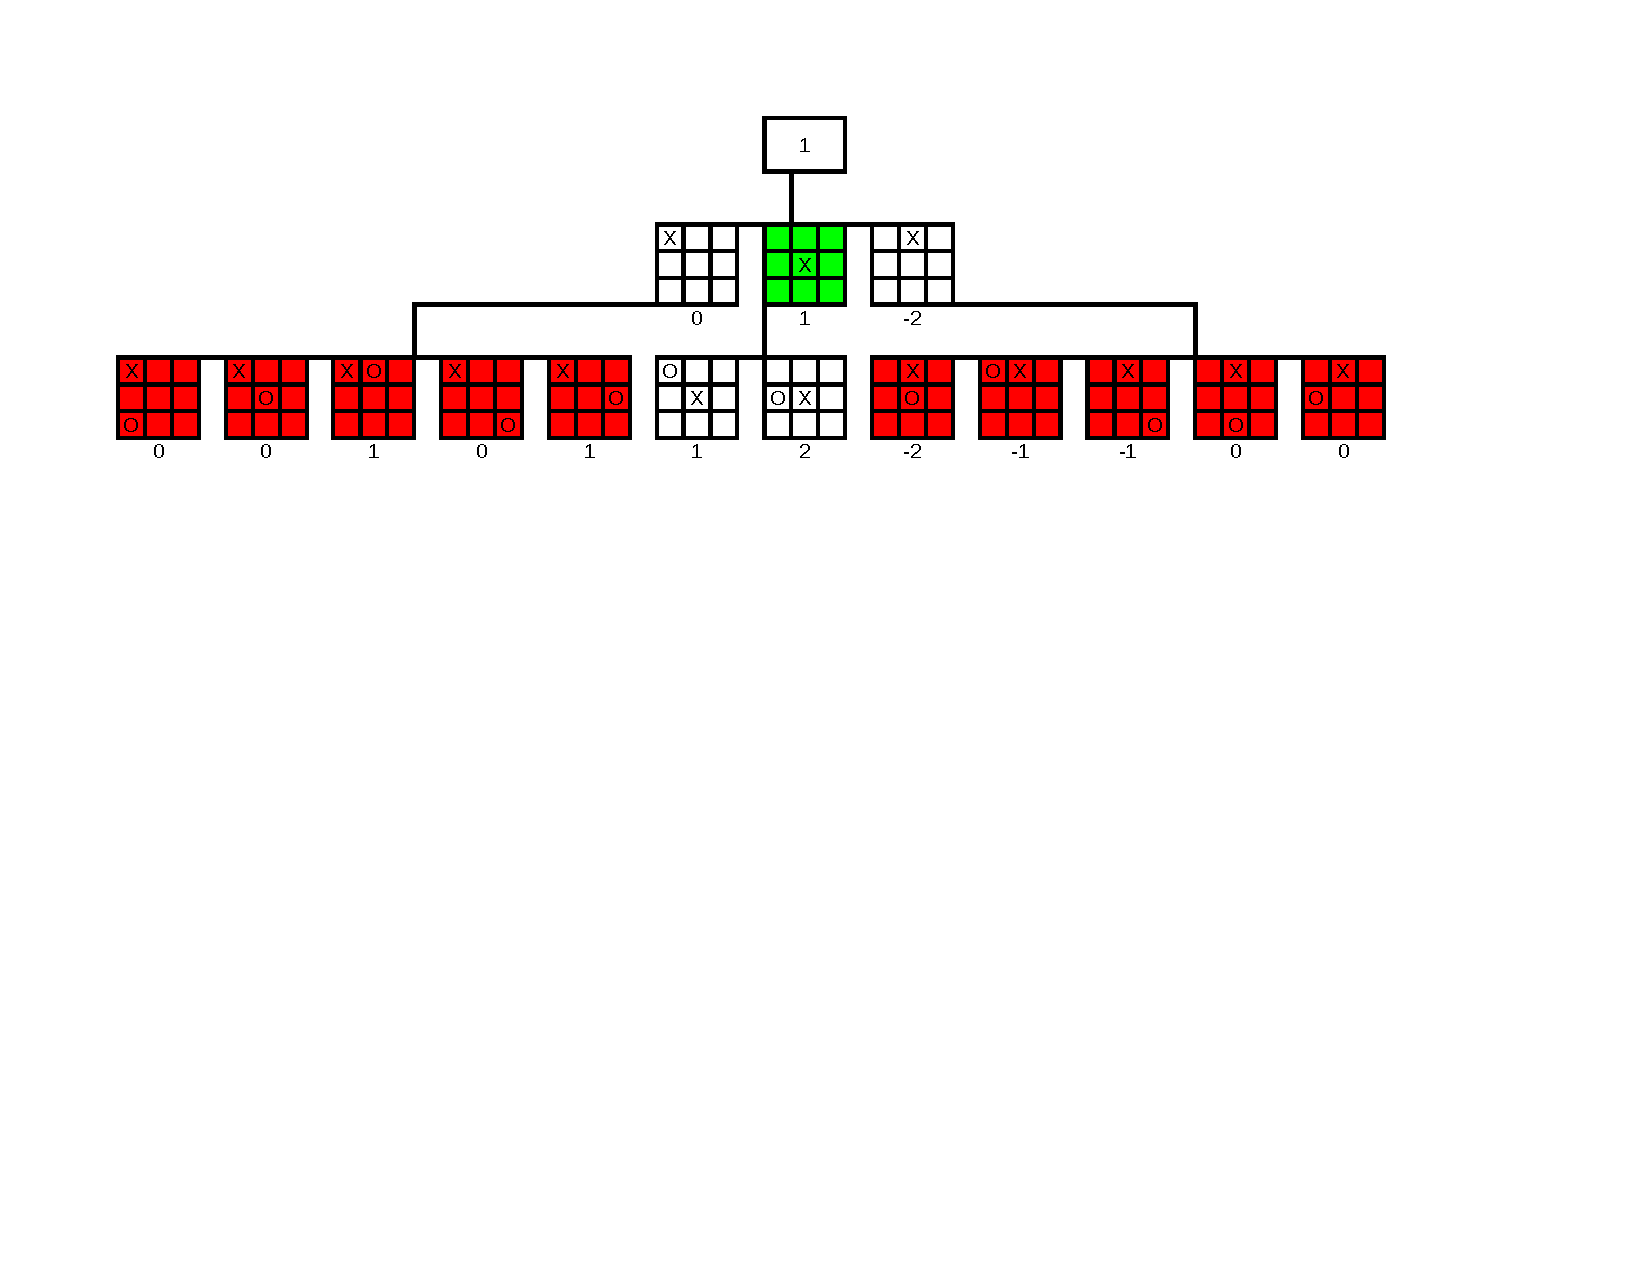
\includepdf{assignment3ABTree.pdf}
\end{document}